Prova di testo di capitolo. Vorrei citare qui tutta l'opera omnia di~\cite{IEEE:1990,WIKI:INTEROP,BOX:1997,AHL:1996}.

\begin{figure}[tbp] 
\begin{center}
\begin{tabular}{c @{\hspace{1em}} c}
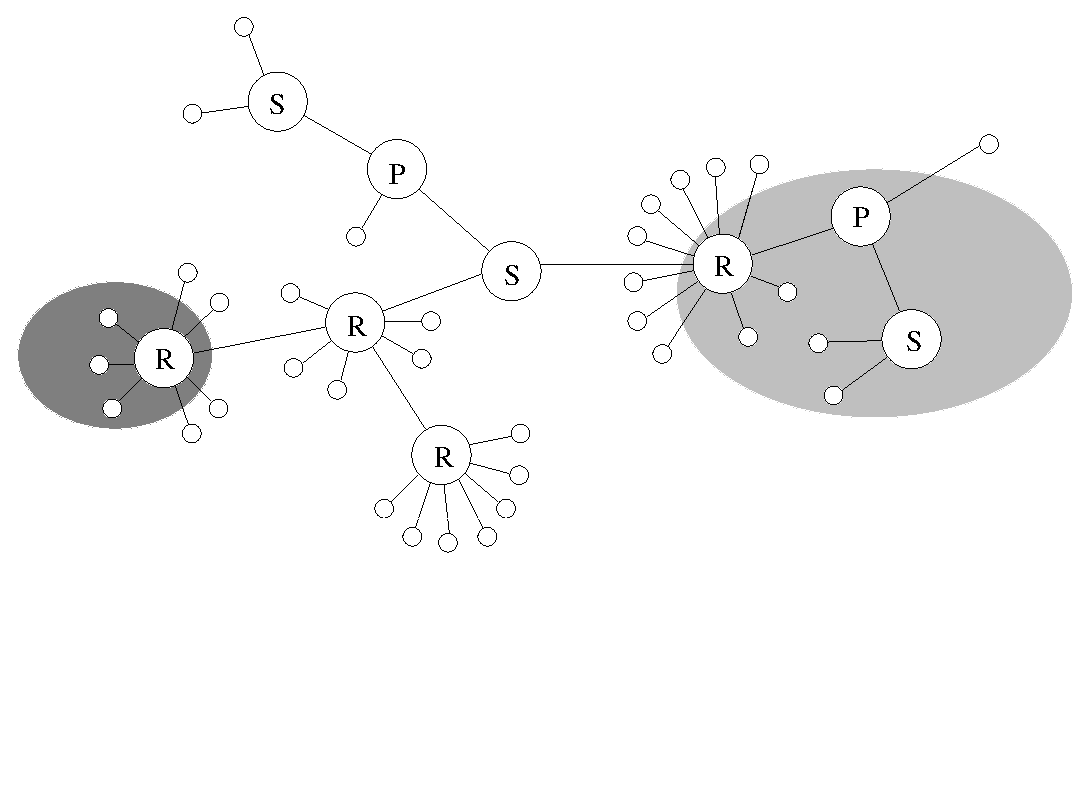
\includegraphics[width=8cm]{figure/esempio-figura-1.eps} &
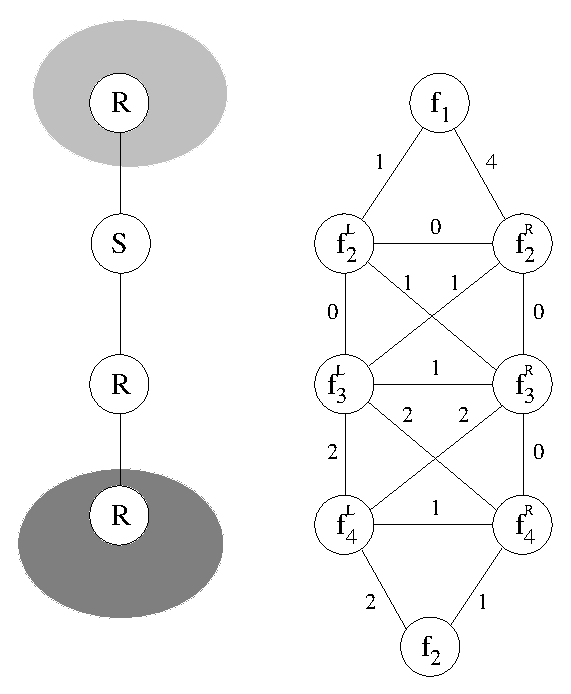
\includegraphics[width=5.5cm]{figure/esempio-figura-2.eps} \\
 (a) & (b)
\end{tabular}
\end{center}
\caption{SPQR-tree di un grafo. (a) L'albero di allocazione della faccia esterna. (b) Il cammino notevole di cui si parla tanto nella Sezione~\ref{se:prima-sezione}.} \label{fig:figura-doppia}
\end{figure}

Come si evince dalle Figure~\ref{fig:figura-doppia}.a e~\ref{fig:figura-doppia}.b non si capisce molto.

\section{La tecnologia Blockchain} % La storia non Nakamoto ma con Napster e il peer2peer 

    \subsection{La vendita del sogno}

    \subsection{Il rovescio della medaglia}

    La macchina infinita di Vitalik (per Etherium) è costruita in che modo?
    %
    Ci interessa sapere come la macchina è costruita perché, in modo molto McLuhanistiano, la macchina forma l'ambiente attorno ad essa. 
    %
    Una \textbf{Blockchain} è composta da due grandi componenti fondamentali: il ledger (libro mastro) e il meccanismo di consenso. 
    %
    Tutte le blockchain attualmente popolari utilizzano un append-only ledger, cioè una nuovo nodo al ledger si aggiunte in coda alla catena e una volta aggiunto è di sola lettura.
    % Questo standard si utilizza solitamente per le attività di log. La blockchain è un'enorme log di transazioni ahahah
    La particolarità è che è decentralizzata, cioè ogni partecipanete elettivo dispone di una completa copia di tutte le transazioni ed è qui che entra in gioco il meccanismo di consenso.
    %
    Tutti i partecipanti validanti, chiamati nodi, hanno una copia completa del database e nessuna delle copie è considerata la copia autorevole.
    %
    Ed è qui che si usa la proof-of-work, in modo da garantire che qualcuno non utilizzi la stessa moneta due volte.


    \section{Cosa resterà dopo lo scoppio della bolla}

    

    \subsection{Modello di dominio}

    Durante questa fase è stato pensato il modello di dominio per l'applicazione 

    \begin{figure}[!ht]
        \centering
        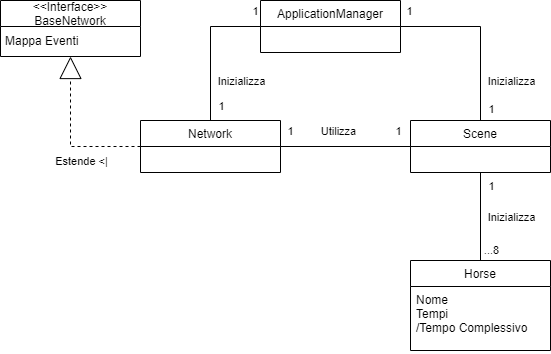
\includegraphics[height=7.5cm]{figure/Modello_di_Dominio_Metarace.png}
        \caption{Modello di dominio}
    \end{figure}

    

    \section{L'elaborazione}

        I requisiti trovati per la prima iterazione sono:
        \begin{itemize}[-]
            \item Implementare uno scenario di base in cui delle mesh basilari percorrono un percorso rettilinio sulla base di un insieme finito di tempi
            \item Implementare una serie di operazioni di sistema legate ad eventi riguardanti la connessione, la partenza e l'arrivo dei gareggianti.
            \item Nello scenario iniziale non c'è una telecamera che segue la scena ne un'interfaccia utente
            \item Il gioco viene eseguito come una simulazione che non richiede alcun input dell'utente
        \end{itemize}

        \begin{lstlisting}[ caption = Sezione del file header della classe SceneController dove vengono istanziate tutte le funzioni associate ai delegate del NetworkActor]
            UCLASS()
            class Metarace AMetaraceSceneController : public AActor
            {
                GENERATED_BODY()
            public:
                void PlayerJoined(const UPlayerJoinedEventDTO* PlayerJoinedEventDto);
                void StartingGrid(const UStartingGridEventDTO* StartingGridEventDto);
                void InitRace(const URaceEventDTO* StartRaceEventDto);
                void StartRace();
                void ShowAvailableRaceFormats(const UAvailableRacesFormatsEventDTO* AvailableRacesFormatsEventDto);
                void AnotherPlayerJoined(const UAnotherPlayerJoinedEventDTO* AnotherPlayerJoinedEventDto);
                void ShowCountDown(const UCountdownEventDTO* CountdownEventDto);
                void SendEndRace();
                void OnLeaderboardEvent(const ULeaderboardEventDTO* LeaderboardEventDto);
            }
                \end{lstlisting}